% Created 2015-01-28 mié 22:18
\documentclass[xcolor={usenames,svgnames,dvipsnames}]{beamer}
\usepackage[utf8]{inputenc}
\usepackage[T1]{fontenc}
\usepackage{fixltx2e}
\usepackage{graphicx}
\usepackage{longtable}
\usepackage{float}
\usepackage{wrapfig}
\usepackage{rotating}
\usepackage[normalem]{ulem}
\usepackage{amsmath}
\usepackage{textcomp}
\usepackage{marvosym}
\usepackage{wasysym}
\usepackage{amssymb}
\usepackage{hyperref}
\tolerance=1000
\usepackage{color}
\usepackage{listings}
\usepackage{mathpazo}
\usepackage{gensymb}
\usepackage{amsmath}
\bibliographystyle{plain}
\AtBeginSubsection[]{\begin{frame}[plain]\tableofcontents[currentsubsection,sectionstyle=show/shaded,subsectionstyle=show/shaded/hide]\end{frame}}
\AtBeginSection[]{\begin{frame}[plain]\tableofcontents[currentsection,hideallsubsections]\end{frame}}
\usepackage[emulate=units]{siunitx}
\sisetup{per=fraction, fraction=nice, decimalsymbol=comma}
\newunit{\wattpeak}{Wp}
\newunit{\watthour}{Wh}
\newunit{\amperehour}{Ah}
\hypersetup{colorlinks=true, linkcolor=Blue, urlcolor=Blue}
\setbeamercolor{alerted text}{fg=red!50!black} \setbeamerfont{alerted text}{series=\bfseries}
\usetheme[hideothersubsections]{Goettingen}
\usecolortheme{rose}
\usefonttheme{serif}
\author{Oscar Perpiñán Lamigueiro \\ \url{http://oscarperpinan.github.io}}
\date{}
\title{SFCR: Seguridad Eléctrica}
\hypersetup{
  pdfkeywords={},
  pdfsubject={},
  pdfcreator={Emacs 24.4.1 (Org mode 8.2.7c)}}
\begin{document}

\maketitle


\section{Definiciones}
\label{sec-1}

\begin{frame}[label=sec-1-0-1]{Contacto Directo e Indirecto}
\begin{description}
\item[{Contacto Directo:}] contacto de personas o animales con partes
activas de los materiales y equipos

\item[{Contacto Indirecto:}] contacto de personas o animales con partes que
se han puesto bajo tensión como resultado de un fallo de aislamiento.

\item[{Partes Activas:}] Conductores y piezas conductoras bajo tensión en
servicio normal. Incluyen el conductor neutro o compensador y las
partes a ellos conectadas.
\end{description}
\end{frame}

\begin{frame}[label=sec-1-0-2]{Masa y Tierra}
\begin{description}
\item[{Masa:}] Conjunto de las partes metálicas de un aparato que, en
condiciones normales, están aisladas de las partes activas.

\item[{Tierra:}] Masa conductora de la tierra en la que el potencial
eléctrico en cada punto se toma, convencionalmente, igual a cero.

\item[{Toma de tierra:}] Electrodo, o conjunto de electrodos, en contacto
con el suelo y que asegura la conexión eléctrica con el mismo.
\end{description}
\end{frame}

\begin{frame}[label=sec-1-0-3]{Clases de materiales}
\begin{description}
\item[{Material de clase 0:}] Material en el cual la protección contra el
choque eléctrico se basa en el aislamiento principal; lo que implica
que no existe ninguna disposición prevista para la conexión de las
partes activas accesibles, si las hay, a un conductor de protección
que forme parte del cableado fijo de la instalación. La protección en
caso de defecto en el aislamiento principal depende del entorno.
\end{description}
\end{frame}

\begin{frame}[label=sec-1-0-4]{Clases de materiales}
\begin{description}
\item[{Material de clase I:}] la protección contra el choque eléctrico no
se basa únicamente en el aislamiento principal, sino que comporta una
medida de seguridad complementaria en forma de medios de conexión de
las partes conductoras accesibles a un conductor de protección puesto
a tierra, que forma parte del cableado fijo de la instalación, de
forma tal que las partes conductoras accesibles no puedan presentar
tensiones peligrosas.
\end{description}
\end{frame}

\begin{frame}[label=sec-1-0-5]{Clases de materiales}
\begin{description}
\item[{Material de clase II:}] la protección comporta medidas de seguridad
complementarias, tales como el doble aislamiento o aislamiento
reforzado. Estas medidas no suponen la utilización de puesta a tierra
para la protección y no dependen de las condiciones de la
instalación. Este material debe estar alimentado por cables con doble
aislamiento o con aislamiento reforzado.

\item[{Material de clase III:}] la protección no se basa en la alimentación
a muy baja tensión y en el cual no se producen tensiones superiores a
50 V en c.a. ó a 75V en c.c.
\end{description}
\end{frame}

\begin{frame}[label=sec-1-0-6]{Tensión de contacto}
\begin{description}
\item[{Tensión de contacto:}] Tensión que aparece entre partes accesibles
simultáneamente, al ocurrir un fallo de aislamiento. Por convenio
este término solo se utiliza en relación con la protección contra
contactos indirectos.\\
   En ciertos casos el valor de la tensión de contacto puede resultar
influido notablemente por la impedancia que presenta la persona en
contacto con esas partes.
\end{description}
\end{frame}

\begin{frame}[label=sec-1-0-7]{Tensión de defecto}
\begin{description}
\item[{Tensión de defecto:}] Tensión que aparece a causa de un defecto de
aislamiento, entre dos masas, entre una masa y un elemento conductor,
o entre una masa y una toma de tierra de referencia, es decir, un
punto en el que el potencial no se modifica al quedar la masa en
tensión.
\end{description}
\end{frame}

\begin{frame}[label=sec-1-0-8]{Esquemas de conexión a tierra}
\begin{description}
\item[{Primera letra:}] conexión de alimentación y tierra

\begin{description}
\item[{T=}] conexión directa de un punto de alimentación a tierra.

\item[{I=}] aislamiento de todas las partes activas respecto a tierra
\end{description}

\item[{Segunda letra:}] conexión de masas con tierra

\begin{description}
\item[{T=}] masas conectadas directamente a tierra, independientemente
de conexión de alimentación

\item[{N=}] masas conectadas directamente a punto de alimentación puesto
a tierra (en alterna, normalmente el neutro)
\end{description}
\end{description}
\end{frame}

\begin{frame}[label=sec-1-0-9]{Esquemas de conexión a tierra}
\begin{description}
\item[{TT:}] en alterna, neutro puesto a tierra y masas a tierra, pero de
forma independiente.\\
   Instalaciones receptoras en una red de distribución pública de BT.

\item[{TN:}] en alterna, neutro puesto a tierra, y masas conectadas al
neutro (directamente o a través de un conductor de protección).

\item[{IT:}] todos los conductores activos aislados de tierra, y masas
conectadas a tierra.\\
   Esquema habitual en zona del generador FV en SFCR europeos.
\end{description}
\end{frame}

\begin{frame}[label=sec-1-0-10]{Esquemas de conexión a tierra}
En un sistema fotovoltaico es de uso común que el esquema de tierra sea
\alert{IT en la zona del generador fotovoltaico} y \alert{TT a partir de la salida
del inversor}.
\end{frame}

\section{Protección de las personas}
\label{sec-2}

\subsection{Efectos de la corriente eléctrica}
\label{sec-2-1}

\begin{frame}[label=sec-2-1-1]{Intensidad y tiempo de contacto}
\begin{itemize}
\item Hasta 10 mA no genera efectos peligrosos (calambres).

\item Por encima de 500 mA puede producir fibrilación muscular.

\item La \alert{intensidad} que circula \alert{depende de la tensión de contacto y la
resistencia expuesta}.

\begin{itemize}
\item Reducir tensión.

\item Aumentar resistencia (guantes, calzado, aislamiento del suelo)
\end{itemize}
\end{itemize}
\end{frame}

\begin{frame}[label=sec-2-1-2]{Intensidad y tiempo de contacto}
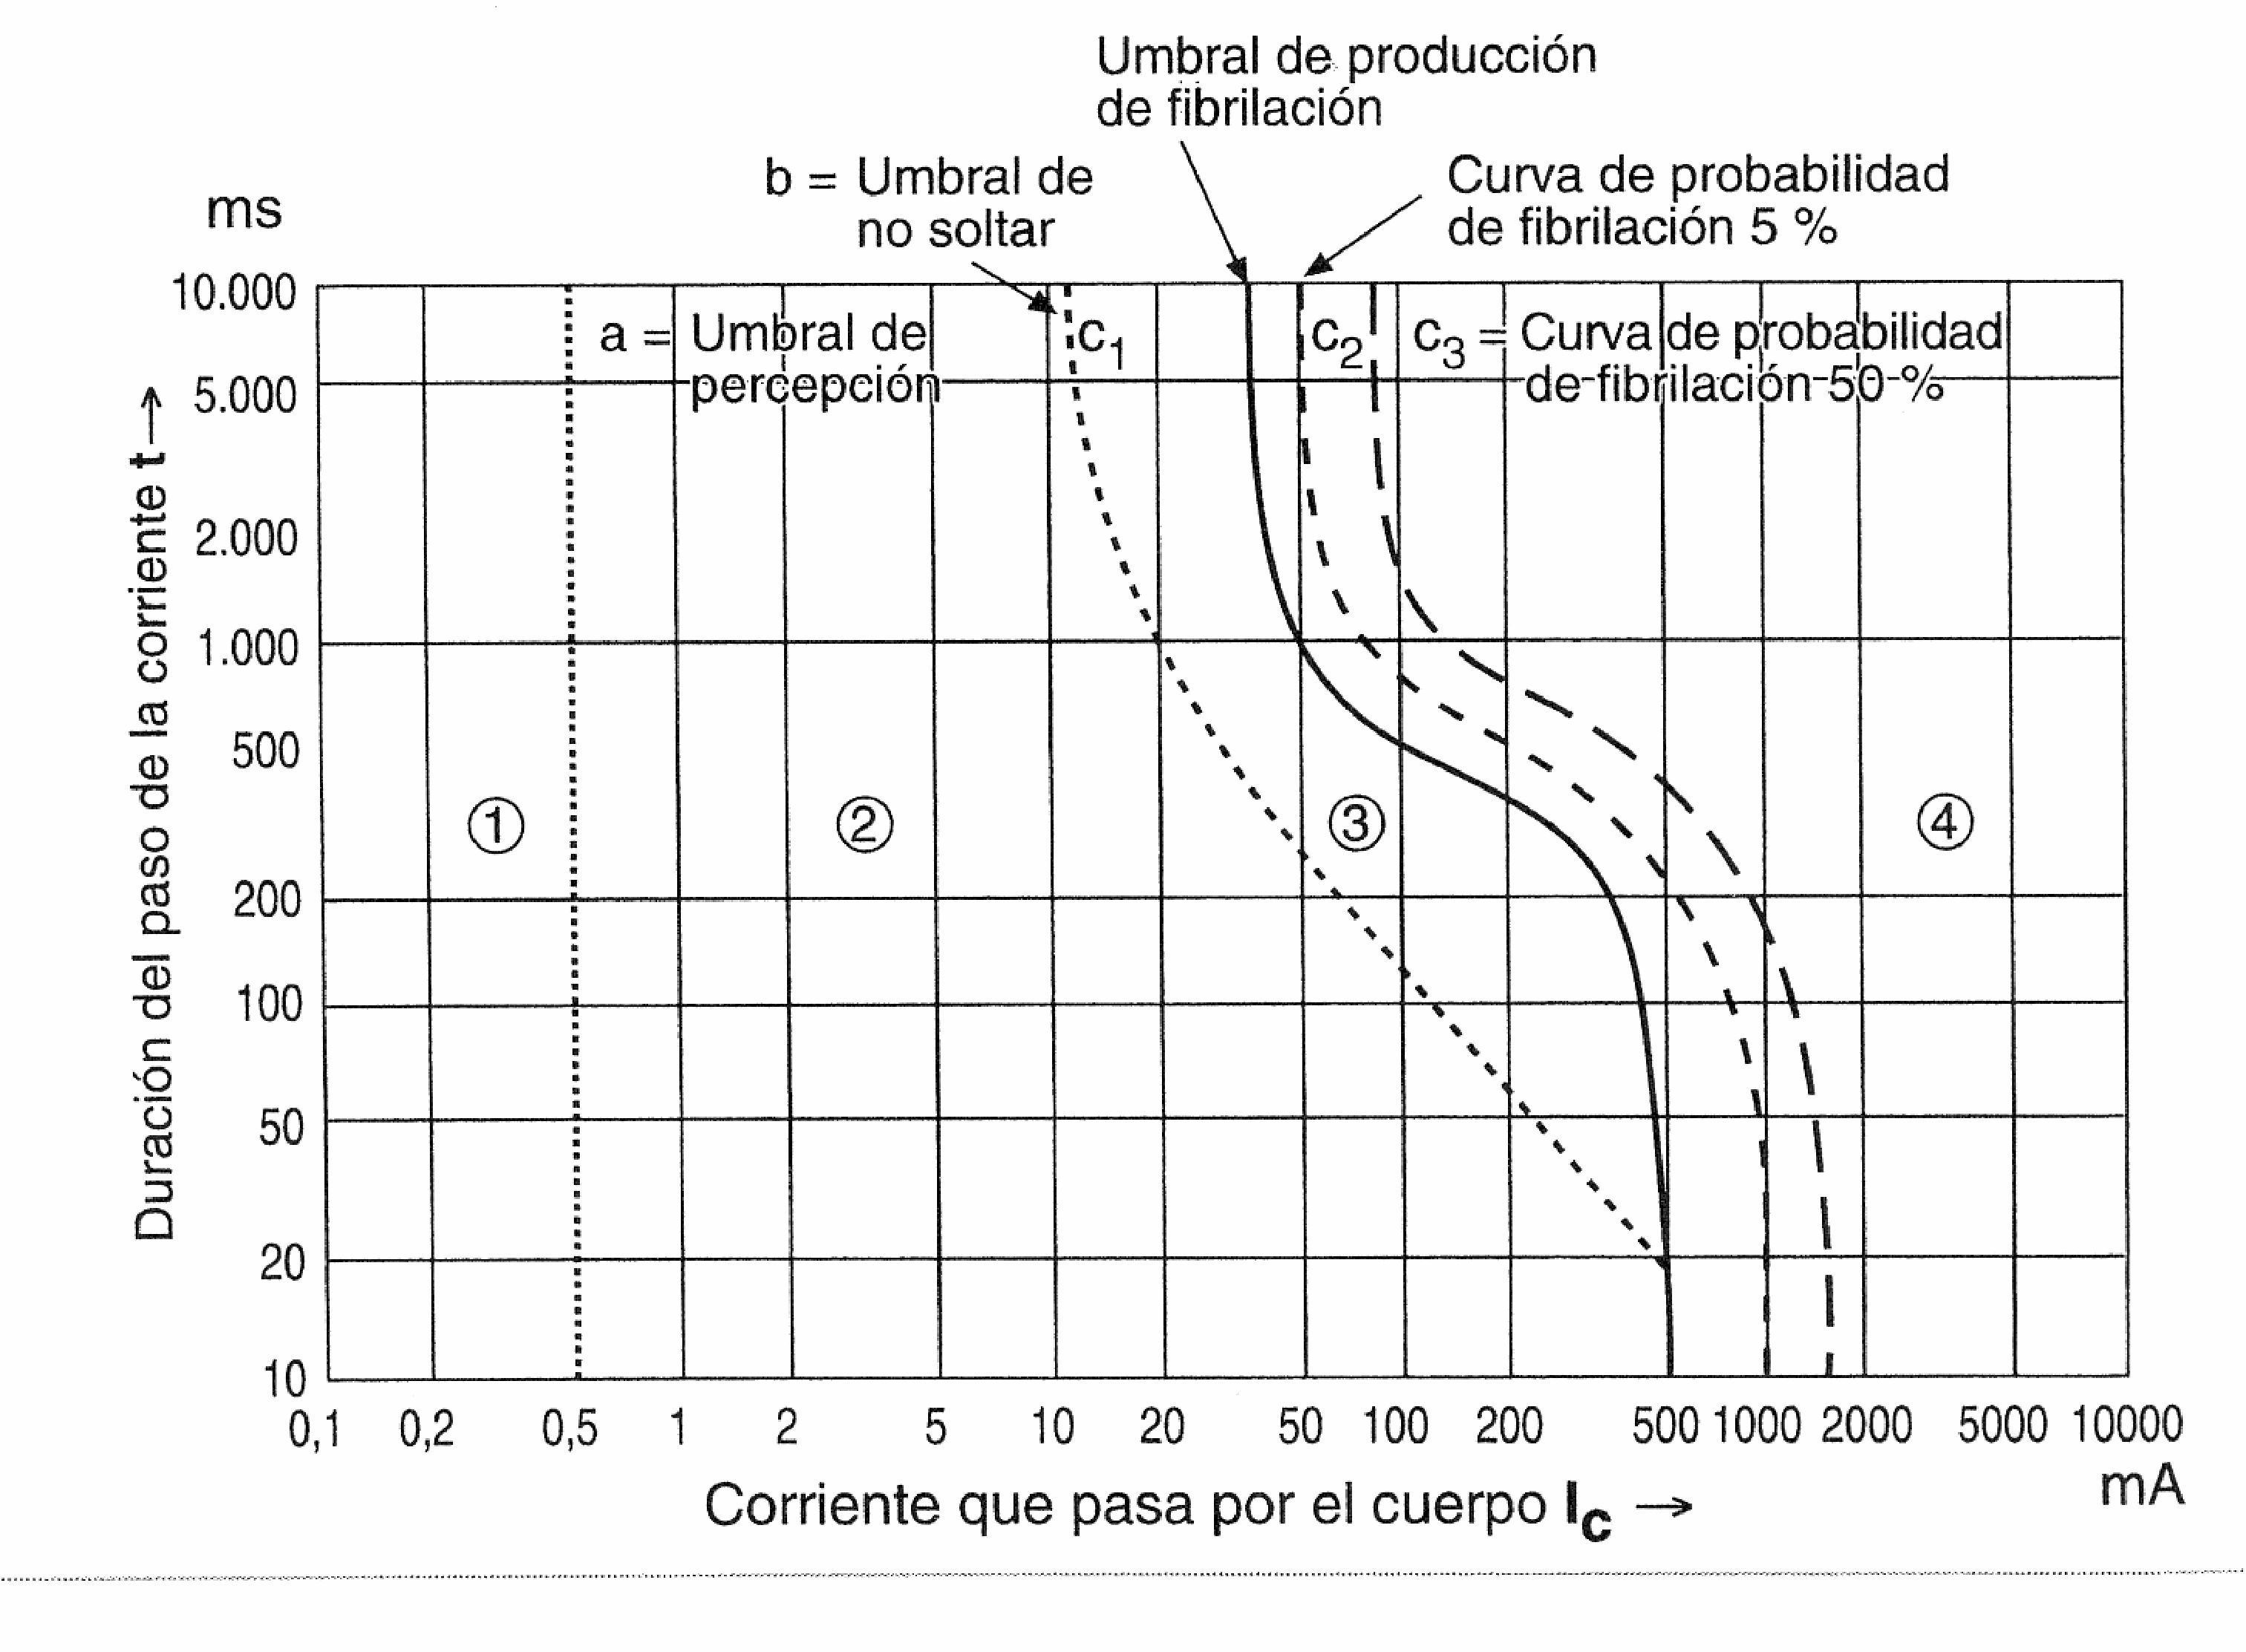
\includegraphics[width=.9\linewidth]{../figs/CurvaIntensidadContactoTiempo.pdf}
\end{frame}

\begin{frame}[label=sec-2-1-3]{Trayectoria de la corriente}
\begin{itemize}
\item La trayectoria se realiza siguiendo la ruta más corta o la de menor
resistencia.

\item Los efectos son más graves si en la trayectoria se encuentran organos
vitales.

\item Además, los efectos dependen de la edad, el sexo, el estado físico,
la fatiga, el miedo\ldots{}
\end{itemize}
\end{frame}

\begin{frame}[label=sec-2-1-4]{Resistencia del cuerpo}
\begin{itemize}
\item No es homogénea: cada parte del cuerpo presenta valores diferentes.

\item No es estable con el tiempo: depende de la duración del contacto y de
la tensión aplicada (disminuye con la tensión!).

\item Depende del estado de la piel, sudoración, estado físico, superficie
de contacto, presión.
\end{itemize}
\end{frame}

\begin{frame}[label=sec-2-1-5]{Frecuencia eléctrica}
\begin{itemize}
\item Continua:

\begin{itemize}
\item Umbral de percepción: 2 mA

\item Umbral control muscular: 75 mA

\item Menos peligrosa que alterna convencional. Puede producir
electrolisis de la sangre.
\end{itemize}

\item Alterna 50 Hz:

\begin{itemize}
\item Umbral de percepción: 0.5 mA

\item Umbral de control muscular: 15 mA
\end{itemize}

\item Alterna 10 kHz:

\begin{itemize}
\item Umbral de percepción: 5 mA

\item Umbral de control muscular: 75 mA

\item Debido al efecto pelicular, los efectos son menores que la alterna
convencional (la corriente circula por la piel, sin atravesar
organos internos).
\end{itemize}
\end{itemize}
\end{frame}

\begin{frame}[label=sec-2-1-6]{Tensión y corriente de seguridad}
\begin{itemize}
\item Se establecen dos condiciones: \alert{emplazamientos secos o húmedos}
(instalaciones de interior); \alert{emplazamientos mojados} (instalaciones
en intemperie).

\item Se define como tensión de seguridad la tensión de contacto máxima
admisible durante al menos cinco segundos. Para emplazamientos secos
es de 120 Vcc y 50 Vca; para \alert{emplazamientos mojados es de 60 Vcc y
24 Vca}.

\item \alert{La corriente máxima admisible se fija en 30 mA para AC y 100 mA para
CC}.
\end{itemize}
\end{frame}

\subsection{Contacto Directo}
\label{sec-2-2}

\begin{frame}[label=sec-2-2-1]{Contacto Directo TT}
$$I_{F,max}=\frac{V_{ocG}}{R_{H}+R_{p}+R_{ts}}$$

\begin{columns}
\begin{column}{5cm\textwidth}
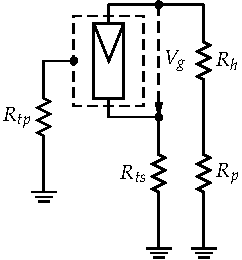
\includegraphics[height=0.5\textheight]{../figs/ContactoDirectoTT.pdf}
\end{column}

\begin{column}{5cm\textwidth}
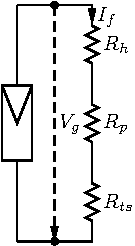
\includegraphics[height=0.5\textheight]{../figs/ContactoDirectoTT_simple.pdf}
\end{column}
\end{columns}
\end{frame}




\begin{frame}[label=sec-2-2-2]{Contacto Directo TN}
$$I_{F,max}=\frac{V_{ocG}}{R_{H}+R_{p}+R_{ts}}$$

\begin{columns}
\begin{column}{5cm\textwidth}
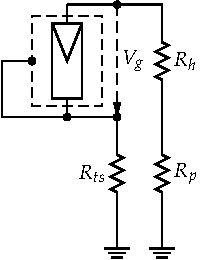
\includegraphics[height=0.5\textheight]{../figs/ContactoDirectoTN.pdf}
\end{column}

\begin{column}{5cm\textwidth}
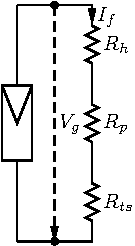
\includegraphics[height=0.5\textheight]{../figs/ContactoDirectoTT_simple.pdf}
\end{column}
\end{columns}
\end{frame}


\begin{frame}[label=sec-2-2-3]{Contacto Directo IT}
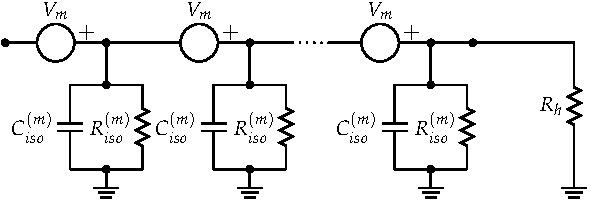
\includegraphics[width=.9\linewidth]{../figs/ContactoDirectoIT_Capacidad.pdf}

$$I_{f}\leq100\, mA\Longrightarrow R_{iso}\geq10\cdot V_{ocG}-R_{H}$$

Se necesitan tensiones de generador superiores a los $\SI{1000}{\volt}$
para producir dolor, y tensiones superiores a los $\SI{3000}{\volt}$
para que exista riesgo por fibrilación.
\end{frame}

\begin{frame}[label=sec-2-2-4]{REBT: Contactos Directos}
Según la ITC-BT-24 las protecciones a utilizar para proteger frente a
contactos directos deben estar \alert{basadas en evitar que una persona pueda
entrar en contacto con las partes activas} de la instalación, e incluye
una protección complementaria cuando las anteriores no consiguen su
objetivo:

\begin{itemize}
\item Protección por \alert{aislamiento de las partes activas}

\item Protección por medio de \alert{barreras o envolventes}

\item Protección por medio de \alert{obstáculos}

\item Protección por puesta \alert{fuera de alcance} por alejamiento

\item Protección complementaria por \alert{dispositivos de corriente
diferencial}-residual
\end{itemize}
\end{frame}

\subsection{Contacto Indirecto}
\label{sec-2-3}

\begin{frame}[label=sec-2-3-1]{Contacto Indirecto TT}
\begin{columns}
\begin{column}{5cm\textwidth}
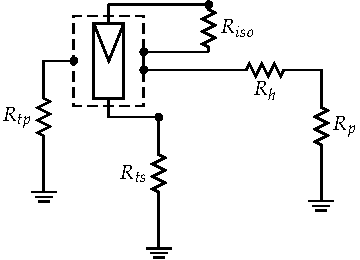
\includegraphics[width=\textwidth]{../figs/ContactoIndirectoTT.pdf}
$$V_{c}\simeq I_{scG}\cdot R_{tp}$$
\end{column}

\begin{column}{5cm\textwidth}
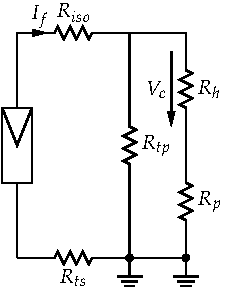
\includegraphics[width=\textwidth]{../figs/ContactoIndirectoTT_simple.pdf}
\end{column}
\end{columns}
\end{frame}


\begin{frame}[label=sec-2-3-2]{Contacto Indirecto TN}
\begin{columns}
\begin{column}{5cm\textwidth}
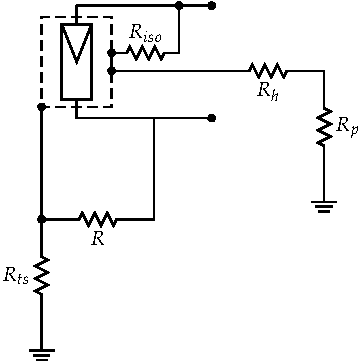
\includegraphics[width=\textwidth]{../figs/ContactoIndirectoTN.pdf}
\end{column}

\begin{column}{5cm\textwidth}
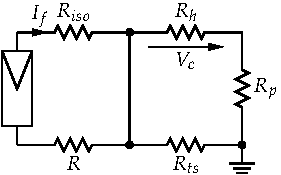
\includegraphics[width=\textwidth]{../figs/ContactoIndirectoTN_simple.pdf}

$$V_{c}=0$$

$$I_{F,max}=\frac{V_{ocG}}{R_{iso}+R}$$
\end{column}
\end{columns}
\end{frame}

\begin{frame}[label=sec-2-3-3]{Contacto Indirecto IT}
\begin{columns}
\begin{column}{5cm\textwidth}
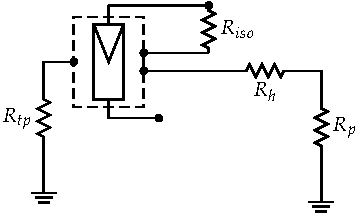
\includegraphics[width=\textwidth]{../figs/ContactoIndirectoIT.pdf}

$$\begin{aligned}
V_{c} & = & 0\\
I_{F} & = & 0\end{aligned}$$
\end{column}

\begin{column}{5cm\textwidth}
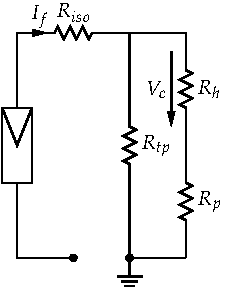
\includegraphics[width=\textwidth]{../figs/ContactoIndirectoIT_simple.pdf}
\end{column}
\end{columns}
\end{frame}


\begin{frame}[label=sec-2-3-4]{REBT: Contactos Indirectos}
Esta misma ITC-BT-24 recoge las formas de protección para contactos
indirectos:

\begin{itemize}
\item Protección por \alert{corte automático de la alimentación}: cuando se
produce el contacto, el objetivo es evitar que la fuente eléctrica
siga alimentando la fuga.

\item Protección por empleo de \alert{equipos de clase II o por aislamiento
equivalente}, con la misión de alcanzar resistencias de aislamiento
de alto valor y estables en el tiempo.

\item \alert{Puesta a tierra}, como camino preferente para conducir la corriente
de fuga y para servir de potencial común para todos los elementos que
entran en contacto con ella.
\end{itemize}
\end{frame}

\section{Puesta a tierra}
\label{sec-3}

\begin{frame}[label=sec-3-0-1]{Resistencia para conexión TT}
$$R_{tp}\leq\frac{V_{max}}{I_{f}}$$

\begin{block}{Ejemplo}
Una instalación fotovoltaica se considera local mojado,
así que $V_{max}=\SI{60}{\volt}$. Al ser corriente continua
$I_{max}=\SI{100}{\milli\ampere}$. Si este generador fotovoltaico
utiliza el esquema TT será $R_{tp}\leq\SI{600}{\ohm}$.
\end{block}
\end{frame}

\begin{frame}[label=sec-3-0-2]{Resistencia para IT con una falta a tierra}
$$R_{tp}\leq\frac{V_{max}}{I_{sc}}$$

\begin{block}{Ejemplo}
Suponiendo $I_{sc}=\SI{150}{\ampere}$, la resistencia de
la puesta a tierra debe ser ahora $R_{tp}\leq\SI{0.4}{\ohm}$.
\end{block}
\end{frame}

\begin{frame}[label=sec-3-0-3]{Práctica común}
Este segundo cálculo arroja un \alert{valor difícilmente alcanzable} en un
terreno con valores de resistividad eléctrica normales \alert{dentro de
ciertos costes razonables}. En general, se suele adoptar como requisito
mínimo $$R_{tp}\leq\frac{V_{max}}{I_{f}}$$ aplicado a la zona de
corriente alterna (por tanto, empleando $V_{max}=\SI{24}{\volt}$ y
$I_{max}=\SI{30}{\milli\ampere}$).

Con este primer resultado se diseña un sistema de puesta a tierra y se
intenta mejorar para alcanzar $$R_{tp}\leq\frac{V_{max}}{I_{sc}}$$
aplicada al generador fotovoltaico.
\end{frame}

\begin{frame}[label=sec-3-0-4]{Cálculo de la resistencia de tierra}
\begin{itemize}
\item \alert{Resistencia de puesta a tierra}: Para una pica vertical $R_{t}=\frac{\rho}{L}$, siendo $\rho$ la resistividad del terreno y $L$ la longitud de la pica.

\item \alert{Resistividad en función del terreno}
\end{itemize}

\begin{center}
\begin{tabular}{ll}
Terrenos cultivables fértiles & $\SI{50}{\ohm\meter}$\\
Terrenos cultivables poco fértiles & $\SI{500}{\ohm\meter}$\\
Suelos pedregosos & $\SI{3000}{\ohm\meter}$\\
\end{tabular}
\end{center}
\end{frame}

\begin{frame}[label=sec-3-0-5]{Cálculo de la resistencia de tierra}
\begin{itemize}
\item \alert{Electrodos en paralelo}: Para mejorar la resistencia de toma de tierra, se utilizan varios electrodos interconectados, situados a distancias del orden de 10 m. De esta forma, \alert{la resistencia equivalente es (aproximadamente) el paralelo de las individuales}.
\end{itemize}

\begin{block}{Por ejemplo}
Para conseguir una $R_{t}=\SI{5}{\ohm}$ en un terreno con
$\rho=\SI{100}{\ohm\meter}$ se deberán utilizar aproximadamente 10 picas de
una longitud de 2 metros (cada una de ellas tendrá una resistencia
$R_{t,i}=\SI{50}{\ohm}$).
\end{block}
\end{frame}

\begin{frame}[label=sec-3-0-6]{Tomas de tierra existentes}
A la hora de realizar puestas a tierra en lugares donde ya existen tomas
a tierra que pertenecen a otras instalaciones eléctricas.

\begin{itemize}
\item Cuando corresponda a la \alert{instalación de Baja Tensión del edificio}
\alert{se utilizará la puesta a tierra existente} para conectar las masas
del sistema fotovoltaico.

\item Cuando corresponde al \alert{neutro de Media Tensión del transformador de
la compañía eléctrica} es necesario \alert{separarse suficientemente} para
no interferir en su funcionamiento. Para terrenos de resistividad no
elevada ($\rho<\SI{100}{\ohm\meter}$), esta condición se cumple para
distancias superiores a $\SI{15}{\meter}$.
\end{itemize}
\end{frame}

\section{Protección de los equipos}
\label{sec-4}

\subsection{Tormentas eléctricas}
\label{sec-4-1}

\begin{frame}[label=sec-4-1-1]{Formación de las tormentas}
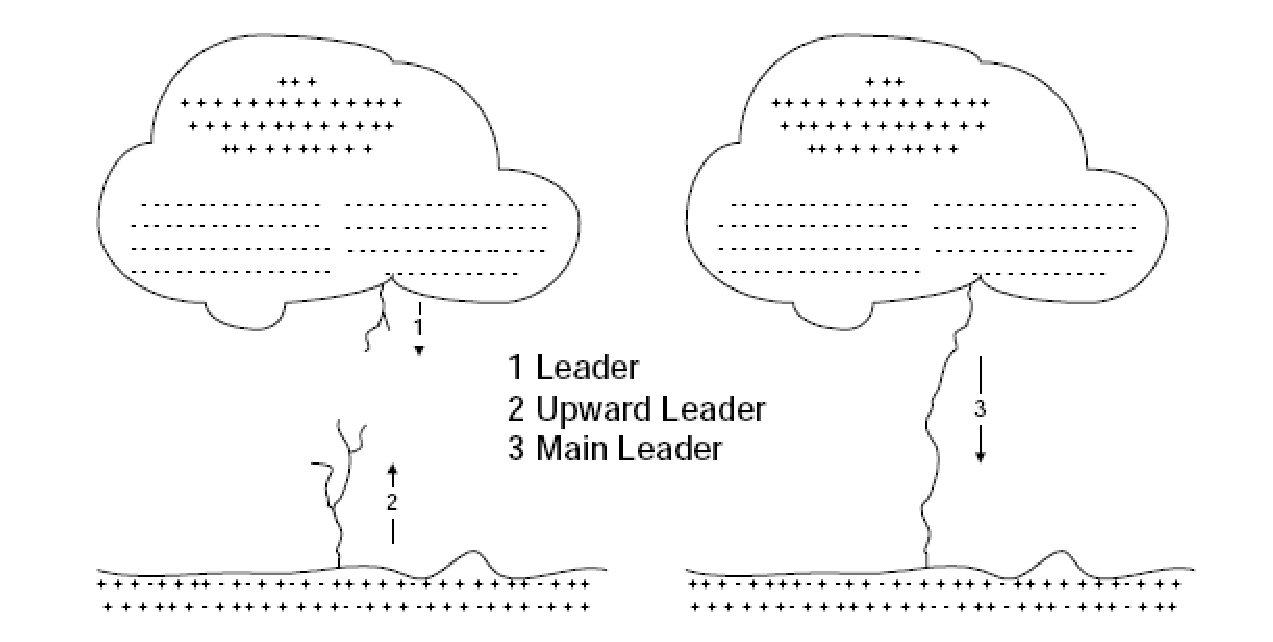
\includegraphics[width=.9\linewidth]{../figs/FormacionTormenta.pdf}
\end{frame}

\begin{frame}[label=sec-4-1-2]{Formación de las tormentas}
\begin{itemize}
\item Dentro de los núcleos tormentosos, las cargas positivas ascienden a
las capas superiores de las nubes. Esta separación de cargas produce
un campo eléctrico.

\item Por otra parte, las cargas negativas de las capas inferiores atraen
las cargas positivas en superficie terrestre.

\item Cuando el campo eléctrico interno de la nube alcanza la ruptura del
aire, se producen descargas eléctricas. Esta descarga comienza en la
nube con un trazador descendente hacia la superficie terrestre.
\end{itemize}
\end{frame}

\begin{frame}[label=sec-4-1-3]{Encuentro entre trazadores}
\begin{itemize}
\item Cuando el trazador descendente se acerca a una distancia de entre 10
a 100 m de la tierra, se generan diversos trazadores ascendentes
desde la superficie en busca del trazador descendente.

\item Aquel trazador ascendente que conecta con el descendente cierra la
descarga y determina el lugar del impacto.
\end{itemize}
\end{frame}

\begin{frame}[label=sec-4-1-4]{Influencia de las condiciones locales}
\begin{itemize}
\item La descarga está determinada principalmente por el campo eléctrico
interno de la nube, con una menor influencia debida a las condiciones
de la superficie terrestre.

\item Cuando el trazador se encuentra a una distancia de entre 10 a 100
metros, las condiciones locales suponen una mayor influencia.

\item Las construcciones metálicas de mayor altura (antenas) o superficie
(instalaciones fotovoltaicas) favorecen la formación de trazadores
ascendentes que conecten con el descendente.
\end{itemize}
\end{frame}

\begin{frame}[label=sec-4-1-5]{Influencia de los sistemas fotovoltaicos}
Por tanto, \alert{las instalaciones fotovoltaicas no aumentan la probabilidad
de descargas locales} (determinadas por las nubes), pero una vez que se
producen, son lugares con mayor probabilidad de impacto.
\end{frame}

\begin{frame}[plain,label=sec-4-1-6]{Descarga y campo magnético}

\begin{columns}
\begin{column}{6cm\textwidth}
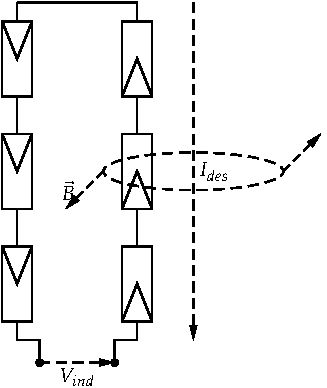
\includegraphics[height=0.8\textheight]{../figs/SobretensionInducida.pdf}
\end{column}
\begin{column}{6cm\textwidth}
\begin{itemize}
\item Una descarga eléctrica supone una corriente de gran valor en un lapso de tiempo muy corto.

\item Esta corriente produce una inducción magnética a su alrededor, también de caracter variable.

\item Un flujo magnético variable produce una fuerza electromotriz entre los extremos del area atravesada.
\end{itemize}
\end{column}
\end{columns}
\end{frame}

\begin{frame}[label=sec-4-1-7]{Factores de influencia}
La fuerza electromotriz inducida depende de:

\begin{itemize}
\item \alert{Valor de la inducción magnética} (depende de la tormenta).

\item \alert{Distancia} de la descarga al sistema (depende principalmente de la
tormenta).

\item \alert{Area efectiva del sistema} (depende del diseñador y del instalador).
\end{itemize}
\end{frame}

\subsection{Protecciones}
\label{sec-4-2}


\begin{frame}[label=sec-4-2-1]{Area y cableado}
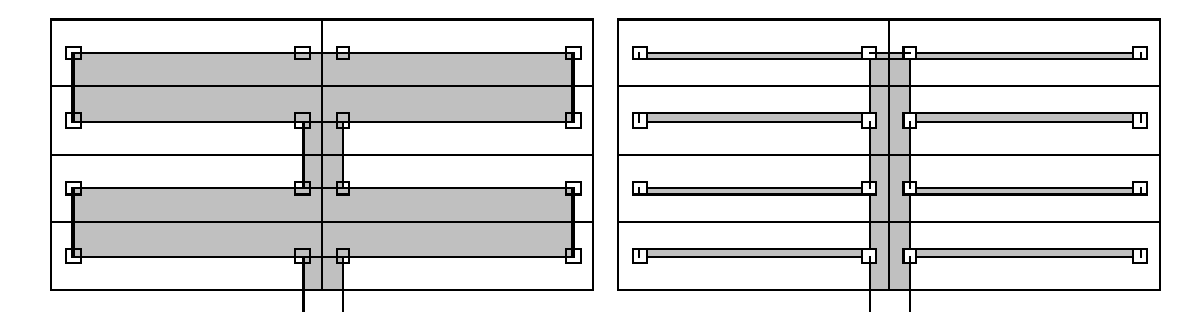
\includegraphics[width=.9\linewidth]{../figs/BucleCableadoOptimo.pdf}
\end{frame}

\begin{frame}[label=sec-4-2-2]{Protección externa}
Un sistema de protección externa contra el rayo se compone de:

\begin{itemize}
\item Terminal aéreo (punta)

\item Conductor(es) de bajada (interconectados)

\item Puesta a tierra.
\end{itemize}
\end{frame}

\begin{frame}[label=sec-4-2-3]{Protección externa}
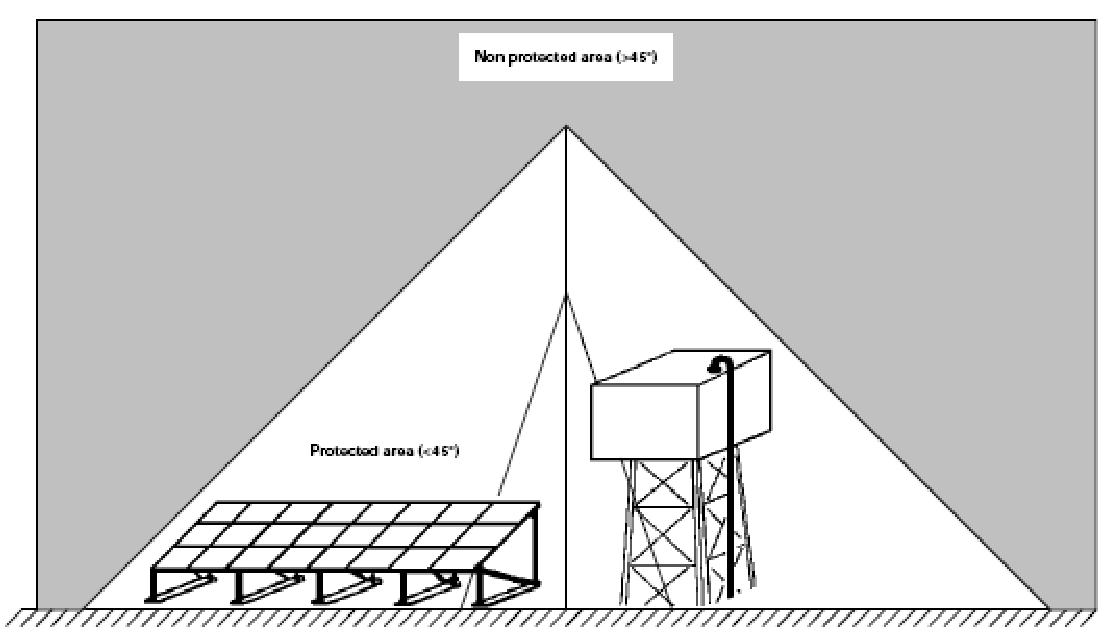
\includegraphics[width=.9\linewidth]{../figs/AreaProteccionPararrayos.pdf}
\end{frame}

\begin{frame}[label=sec-4-2-4]{Protección externa}
\begin{itemize}
\item Se debe calcular una \alert{distancia de seguridad} entre la bajada del
pararrayos y las instalaciones metálicas cercanas.

\item Se asume que una distancia mayor a 1 metro es superior a la distancia
de seguridad.

\item \alert{Si la distancia es inferior a la de seguridad}, el sistema de puesta
a tierra de la protección externa y la estructura metálica deben
\alert{interconectarse} para evitar la existencia de descargas entre
conductores.

\item \alert{Si la distancia es superior a la de seguridad}, los sistemas de
puesta a tierra deben ser \alert{independientes}.
\end{itemize}
\end{frame}

\begin{frame}[label=sec-4-2-5]{Protecciones internas}
\begin{itemize}
\item \alert{Todas las masas deben estar conectadas a un sistema de puesta a
tierra}. En general, la estructura de soporte se conecta directamente
a tierra, pero no el marco de los módulos.

\item En la entrada/salida de cada elemento a proteger se instalan
\alert{supresores de tensión (varistores)} entre conductores activos y
tierra.

\item Es importante tener en cuenta que cuando un varistor actúa, realiza
un cortocircuito entre sus conexiones.
\end{itemize}
\end{frame}


\begin{frame}[label=sec-4-2-6]{Protecciones Internas}
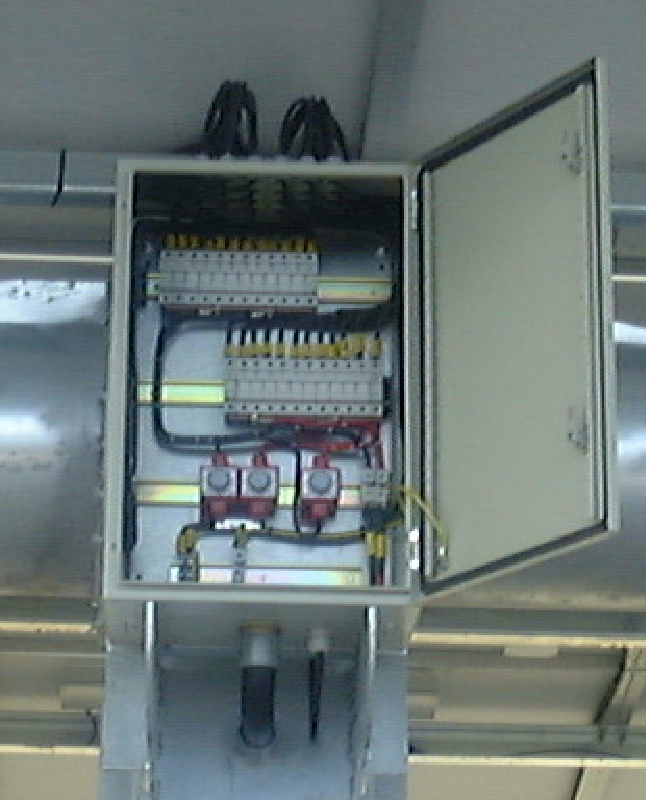
\includegraphics[height=0.8\textheight]{../figs/CajaProteccionesPhotocampa.pdf}
\end{frame}

\begin{frame}[label=sec-4-2-7]{Protecciones Internas}
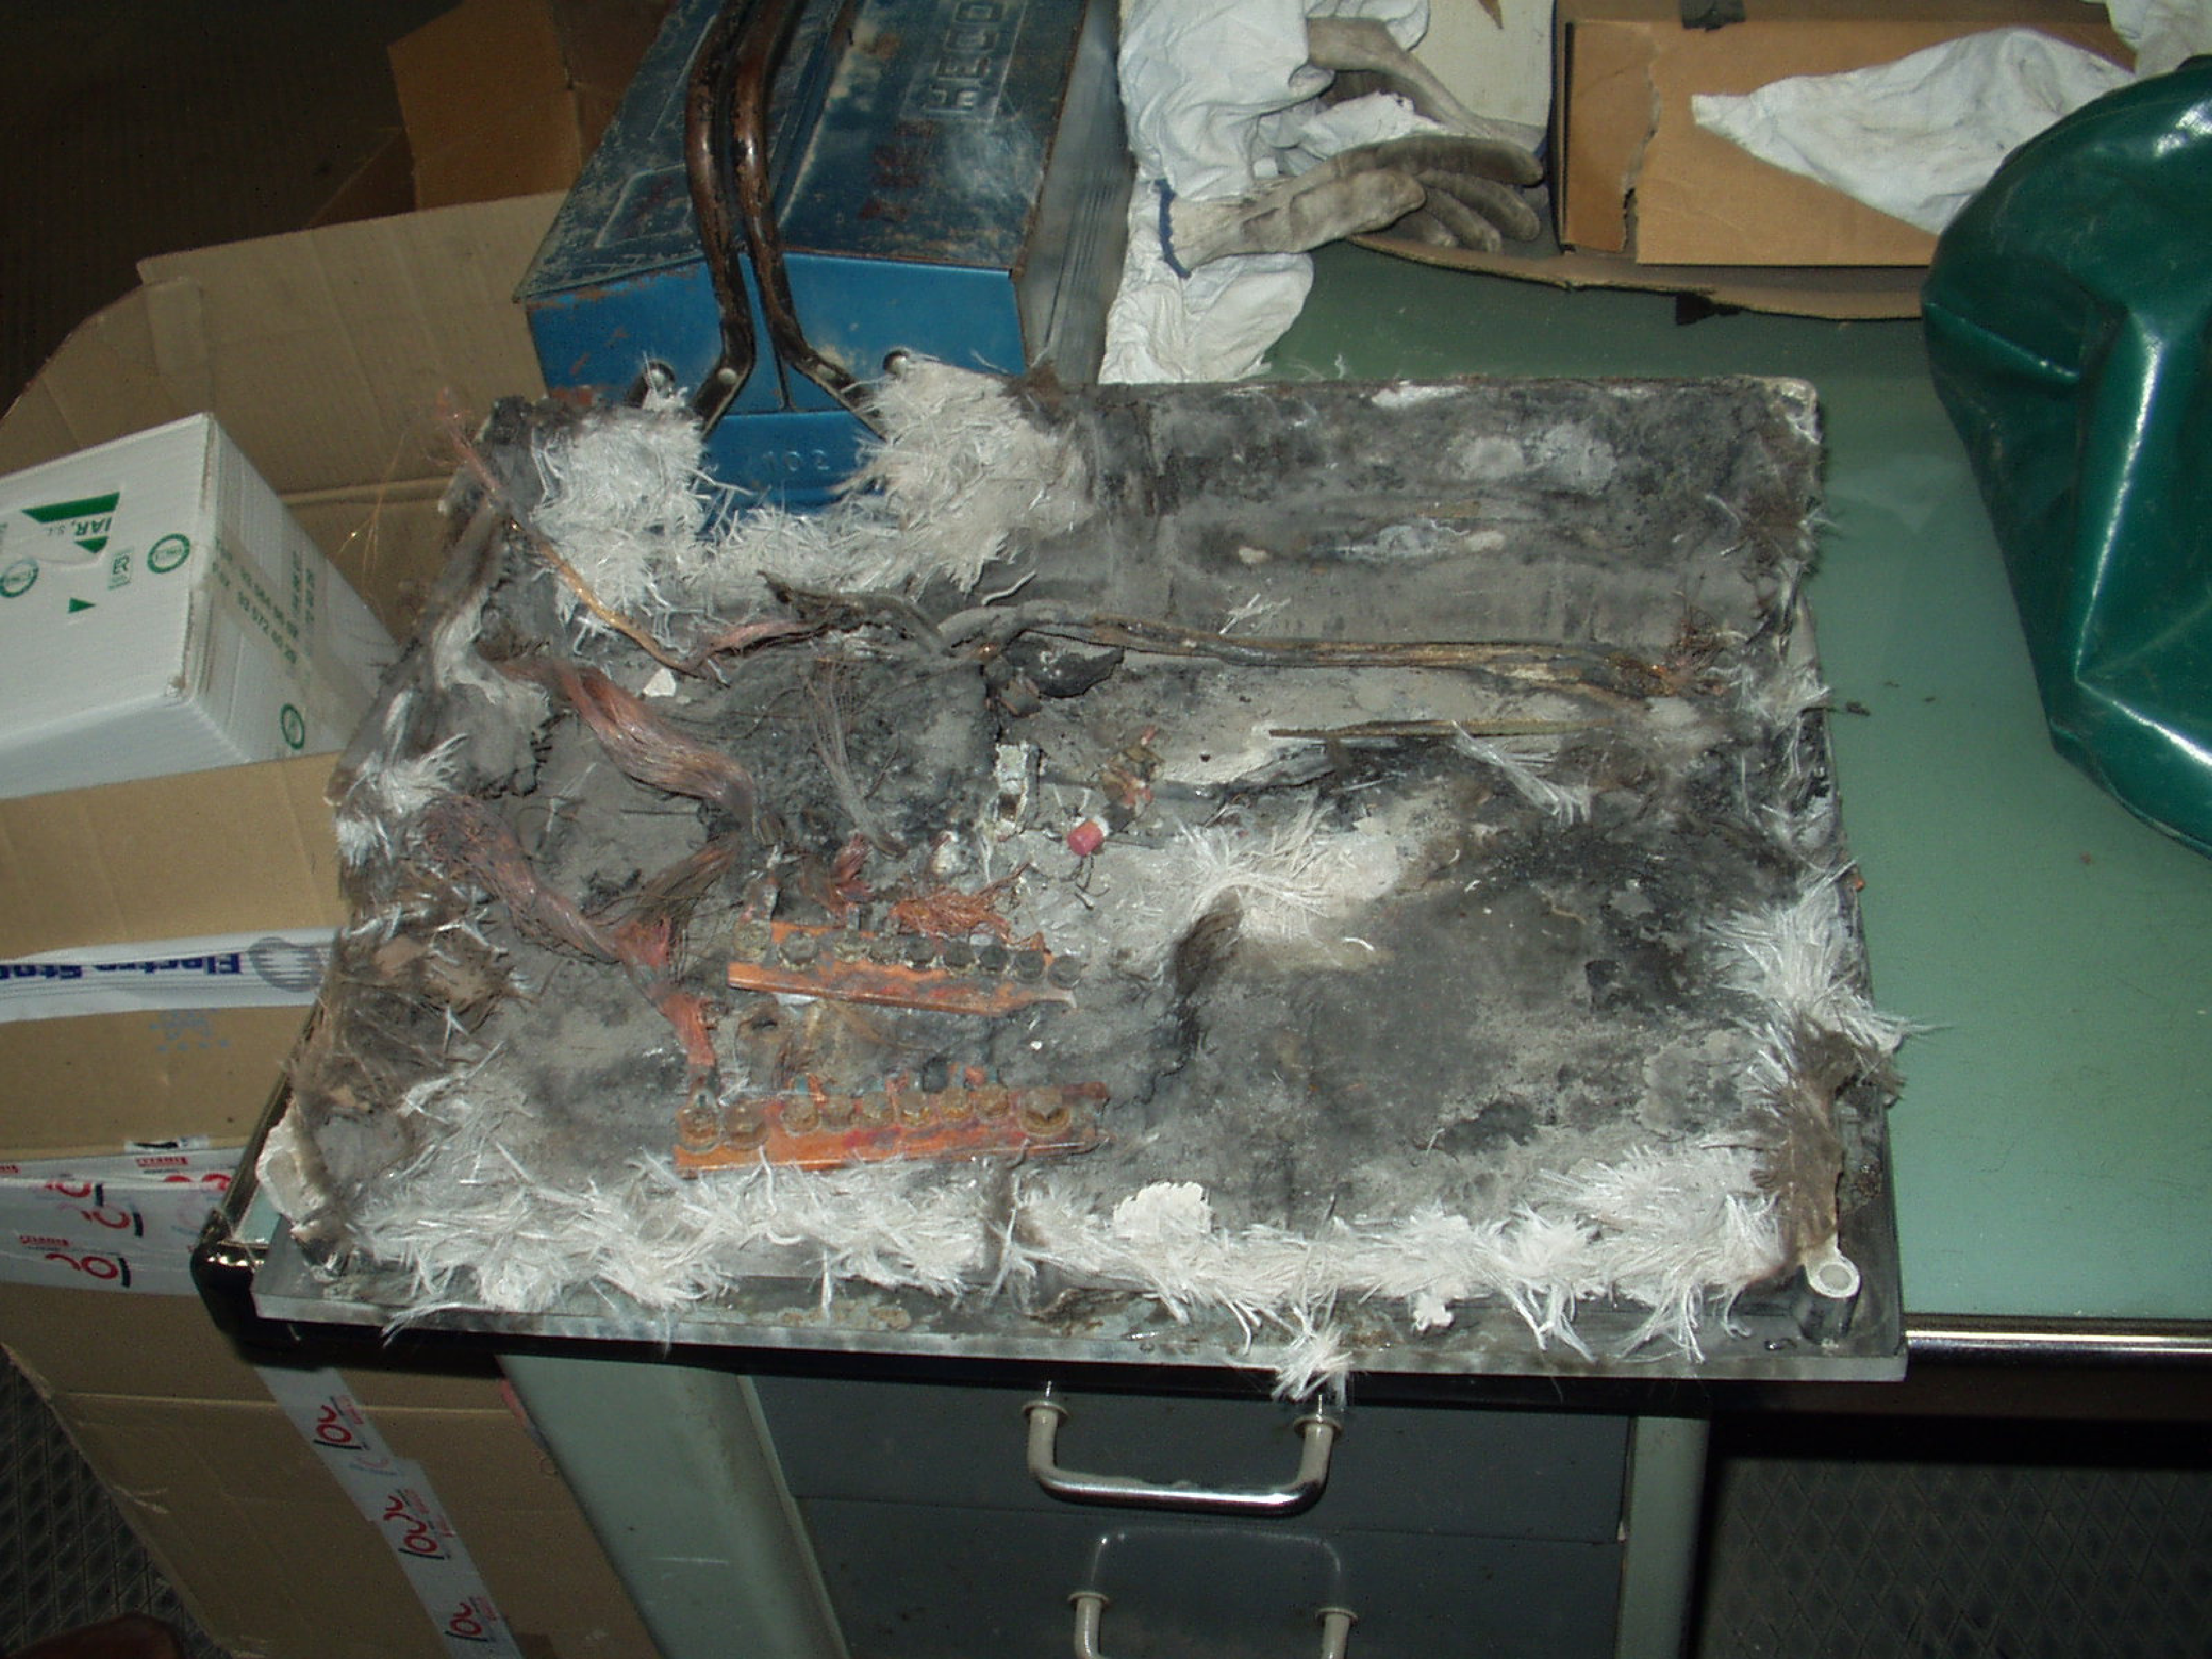
\includegraphics[width=.9\linewidth]{../figs/CajaForumDestruida.pdf}
\end{frame}

\section{Resumen de protecciones}
\label{sec-5}

\begin{frame}[plain,label=sec-5-0-1]{Diagrama Unifilar}
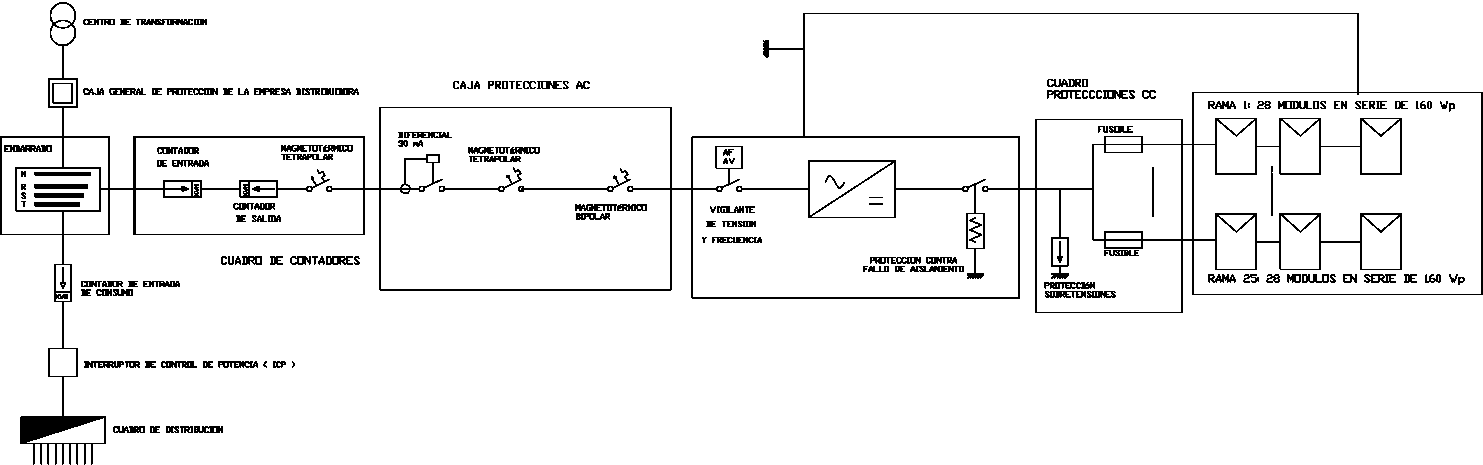
\includegraphics[width=1.2\textwidth]{../figs/UnifilarCR1.pdf}
\end{frame}

\subsection{Circuito DC}
\label{sec-5-1}

\begin{frame}[label=sec-5-1-1]{Tres niveles de protección}
Todo el sistema de protección para sistemas IT se puede concebir en tres
niveles:

\begin{itemize}
\item Nivel 1: Refuerzo del aislamiento de las partes activas.

\item Nivel 2: Sistema de detección de aislamiento.

\item Nivel 3: Puesta a tierra.
\end{itemize}
\end{frame}

\begin{frame}[label=sec-5-1-2]{Nivel 1: Refuerzo del aislamiento de las partes activas.}
\begin{description}
\item[{Configuración flotante del generador:}] se imposibilitan los
accidentes por la aparición de contactos indirectos de primer
contacto.

\item[{Cableado con aislamiento de protección:}] Estos aislamientos
refuerzan la protección contra contactos indirectos.

\item[{Aislamiento galvánico AC-DC:}] Mediante transformadores de devanados
independientes en los inversores se imposibilita el cierre de
corriente de fallo a través del inversor.
\end{description}
\end{frame}

\begin{frame}[label=sec-5-1-3]{Nivel 2: Sistema de detección de aislamiento.}
\begin{description}
\item[{Vigilante de aislamiento:}] Este elemento genera una señal de baja
frecuencia (2 a 5 Hz) para evitar las fugas capacitivas del cableado,
y que inyecta en un polo activo midiendo la corriente de retorno, y
por tanto, la resistencia de aislamiento.

\item[{En caso de pérdida de aislamiento,}] el vigilante ordena el disparo
de los interruptores aislando el campo fotovoltaico afectado. La
orden provoca la desconexión del inversor, el cortocircuito del campo
y la puesta a tierra del mismo.
\end{description}
\end{frame}

\begin{frame}[label=sec-5-1-4]{Nivel 3: Protección en caso de fallo de los niveles 1 y 2:}
\begin{description}
\item[{En caso de fallo de los niveles anteriores}] aún queda la protección
proporcionada por la puesta a tierra directa de todas las masas de la
planta. Gracias a ella se limitara la tensión que con respecto a
tierra puedan adquirir las masas en caso de derivación.
\end{description}
\end{frame}

\begin{frame}[label=sec-5-1-5]{Cortocircuitos}
\begin{itemize}
\item El \alert{cortocircuito} es un punto de trabajo \alert{no peligroso para el
generador fotovoltaico}.

\item El cortocircuito puede, sin embargo, ser \alert{perjudicial para el
inversor}. Como medio de protección se incluyen fusibles de tipo gG
normalizados según EN 60269 en cada polo.

\item Para las personas es \alert{peligrosa la realización o eliminación de un
cortocircuito franco en el campo generador}, por la posibilidad de
que se establezca un arco eléctrico. Es recomendable la \alert{conducción
separada} del positivo y del negativo para evitar cortocircuitos por
pérdida de aislamiento.
\end{itemize}
\end{frame}

\begin{frame}[label=sec-5-1-6]{Fusibles}
\begin{itemize}
\item El \alert{fusible por rama} sirve principalmente como \alert{elemento de
seccionamiento} (facilita las tareas de mantenimiento). Debe elegirse
mediante:

$$\begin{aligned}
   I_{B} & < & I_{n}<I_{z}\\
   I_{2} & < & 1.45\cdot I_{z}\end{aligned}$$

siendo $I_{B}$ la intensidad de diseño de la línea, $I_{n}$ la
intensidad nominal del dispositivo de protección, e $I_{z}$ es la
intensidad admisible por el conductor e $I_{2}$ la intensidad que
asegura efectivamente el funcionamiento del dispositivo de
protección.

\item Suele utilizarse $I_{n}\geq1.25\cdot I_{scG}$ . Para fusibles,
normalmente $I_{2}=1.6\cdot I_{n}$
\end{itemize}
\end{frame}

\begin{frame}[label=sec-5-1-7]{Fusibles}
\begin{itemize}
\item En las instalaciones eléctricas convencionales es frecuente el empleo
de fusibles (y otros elementos de protección) en cascada con poder de
corte creciente en dirección al punto de conexión a red.

\item Esta práctica se basa en que, en la red convencional, la corriente de
cortocircuito es sustancialmente superior a la de operación.
\end{itemize}
\end{frame}

\begin{frame}[label=sec-5-1-8]{Fusibles}
\begin{itemize}
\item Sin embargo, su traslación directa a los sistemas fotovoltaicos
carece de sentido dada la similitud entre ambas corrientes.

\item Aunque puede defenderse su utilidad al permitir el seccionamiento
parcial del generador debe tenerse en cuenta que esta funcionalidad
la ofrece el portafusibles y no el fusible mismo.
\end{itemize}
\end{frame}

\begin{frame}[label=sec-5-1-9]{Sobretensiones}
\begin{itemize}
\item Se protegerá la entrada CC del inversor mediante \alert{varistores}
(dispositivos bipolares de protección clase II), válidos para la
mayoría de equipos conectados a la red.

\item El dispositivo tendrá una tensión de operación marcada por el diseño
del sistema concreto, rango definido entre la tensión de serie para
la menor tensión en el punto de máxima potencia y la mayor tensión de
circuito abierto.
\end{itemize}
\end{frame}

\subsection{Circuito AC}
\label{sec-5-2}

\begin{frame}[label=sec-5-2-1]{Cortocircuitos y sobrecargas}
Según el RD 1663-2000 es necesario incluir un \alert{interruptor general
manual}, que será un interruptor magnetotérmico omnipolar.

Este interruptor, que se ubica en el cuadro de contadores de la
instalación fotovoltaica, será \alert{accesible sólo a la empresa
distribuidora}, con objeto de poder realizar la desconexión manual, que
permita la realización, de forma segura, de labores de mantenimiento en
la red de la compañía eléctrica.
\end{frame}

\begin{frame}[label=sec-5-2-2]{Cortocircuitos y sobrecargas}
\begin{itemize}
\item Esta inaccesibilidad obliga a introducir un \alert{segundo magnetotérmico
omnipolar} en la instalación, de menor intensidad nominal, que será
el que realmente proteja a la instalación AC de las sobrecargas y
cortocircuitos.

\item Este segundo magnetotérmico actuará antes que el interruptor general
manual, salvo cortocircuitos de cierta importancia provenientes de la
red de la compañía.

\item Asimismo, con el fin de dar cierta independencia a las líneas propias
de cada inversor, se utilizará un magnetotérmico de menor corriente
asignada para cada inversor.
\end{itemize}
\end{frame}

\begin{frame}[label=sec-5-2-3]{Cortocircuitos y sobrecargas}
Se utilizarán \alert{magnetotérmicos tipo C}, los utilizados cuando no existen
corrientes de arranque de consumo elevadas, cumpliendo:

$$\begin{aligned}
I_{B} & < & I_{n}<I_{z}\\
I_{2} & < & 1.45\cdot I_{z}\end{aligned}$$

Los interruptores magnetotérmicos normalizados cumplen
$I_{2}=1.45\cdot I_{n}$.
\end{frame}

\begin{frame}[label=sec-5-2-4]{Interruptor diferencial}
\begin{itemize}
\item Un interruptor diferencial está basado en un toroide que enlaza a
todos los conductores. Si existe una corriente de defecto, la
corriente en cada conductor es diferente. Según la sensibilidad del
interruptor, cortará el circuito a partir de un umbral de corriente.

\item Al estar basado en la ley de Faraday (fuerza electromotriz creada un
por un flujo magnético variable), \alert{no funciona en circuitos DC}.
\end{itemize}
\end{frame}

\begin{frame}[label=sec-5-2-5]{Interruptor diferencial}
\begin{itemize}
\item En redes de distribución pública la conexión es TT. La corriente de
fallo cerrará el circuito a través de la puesta a tierra del neutro
del centro de transformación. Por tanto, el diferencial \alert{no} protege
el tramo comprendido entre él y el centro de transformación.
\end{itemize}

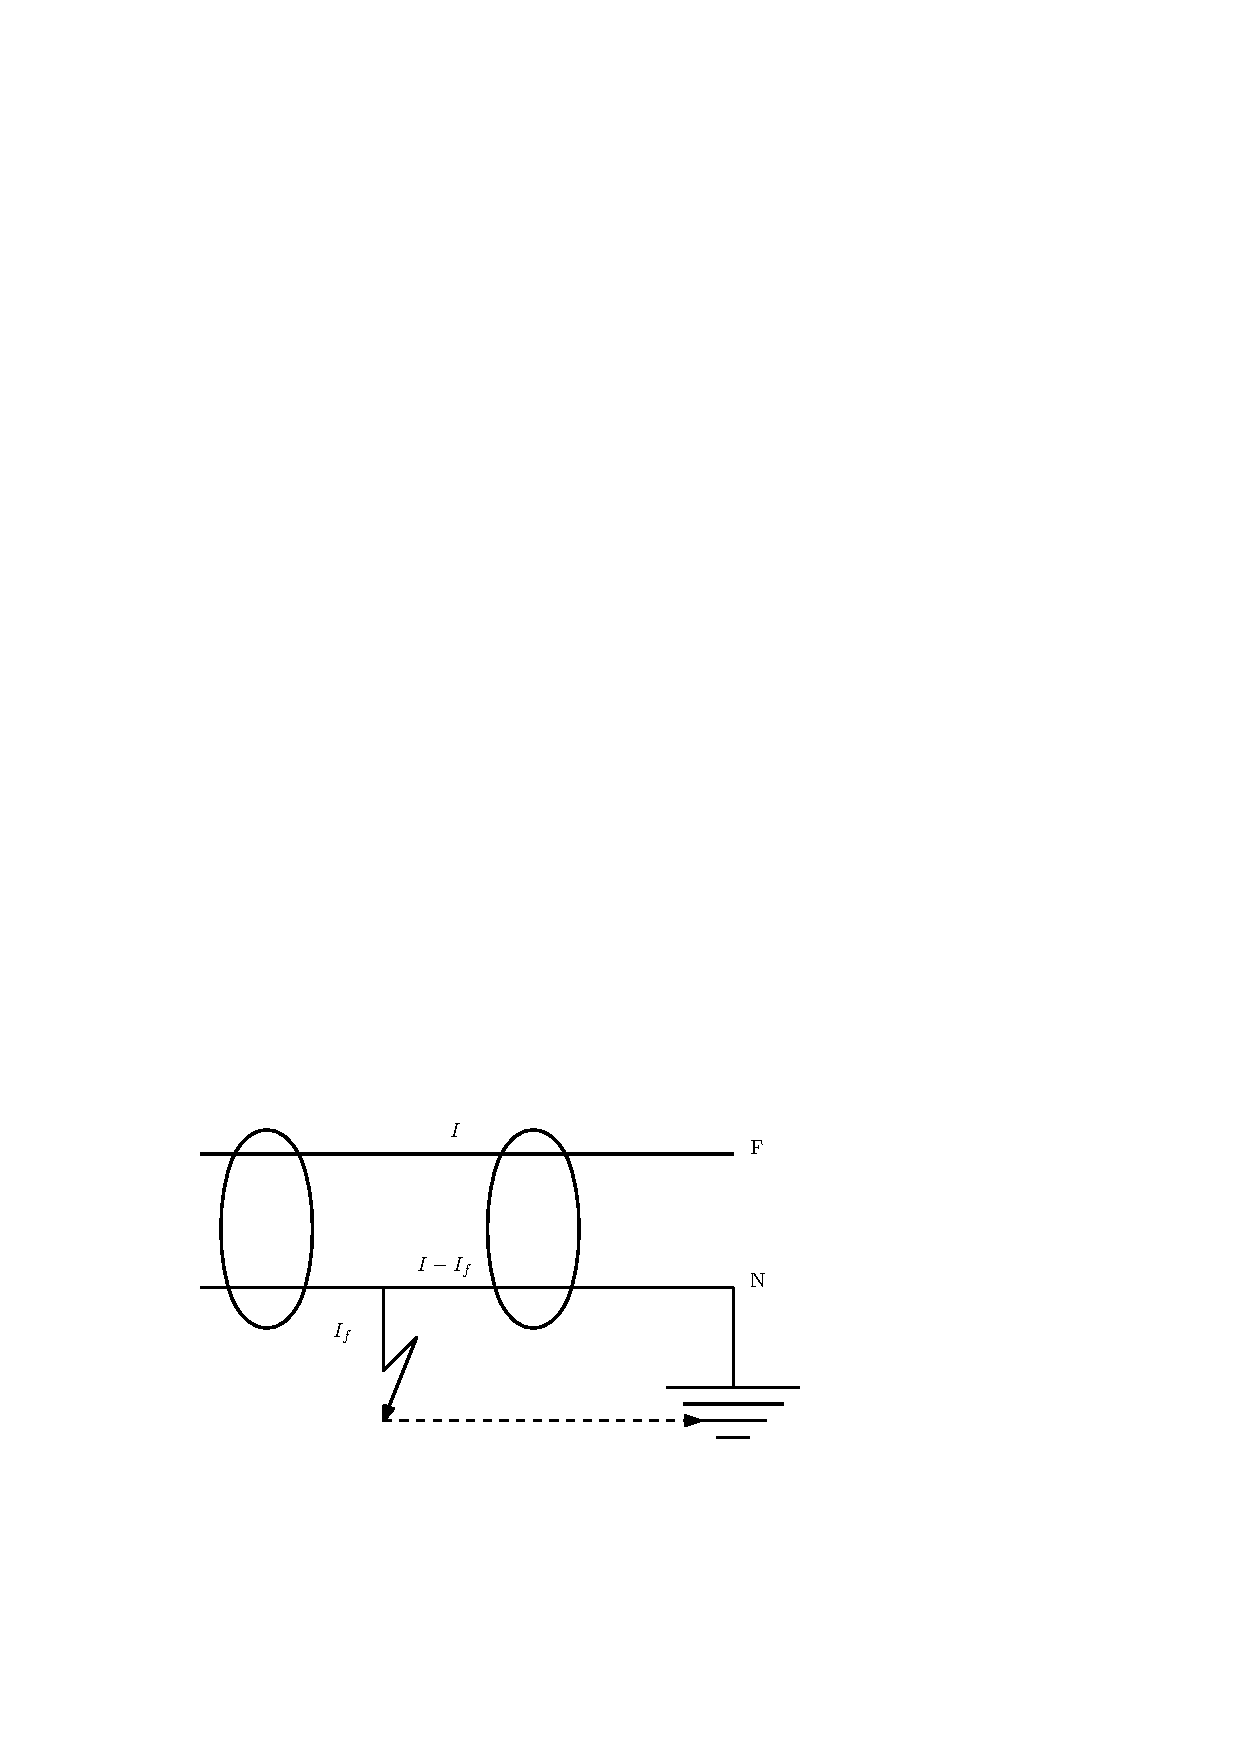
\includegraphics[width=.9\linewidth]{../figs/InterruptorDiferencial.pdf}
\end{frame}

\begin{frame}[label=sec-5-2-6]{Interruptor diferencial}
\begin{itemize}
\item La instalación contará con diferencial de 30 mA de sensibilidad en la
parte CA, para proteger de derivaciones en este circuito.

\item Con el fin de que sólo actúe por fallos a tierra, será de una
corriente asignada superior a la del magnetotérmico de protección.
\end{itemize}
\end{frame}

\begin{frame}[label=sec-5-2-7]{Puesta a tierra}
\begin{itemize}
\item Según RD 1663/2000, en que se fijan las condiciones técnicas para la
conexión de instalaciones fotovoltaicas a la red, \alert{la puesta a
tierra} se realizará de forma que \alert{no altere la de la compañía
eléctrica distribuidora}, con el fin de no transmitir defectos a la
misma.

\item Asimismo, \alert{las masas de la instalación fotovoltaica estarán
conectadas a una tierra independiente de la del neutro} de la empresa
distribuidora de acuerdo con el Reglamento Electrotécnico para Baja
Tensión.
\end{itemize}
\end{frame}
% Emacs 24.4.1 (Org mode 8.2.7c)
\end{document}